
% Default to the notebook output style

    


% Inherit from the specified cell style.




    
\documentclass[11pt]{article}

    
    
    \usepackage[T1]{fontenc}
    % Nicer default font (+ math font) than Computer Modern for most use cases
    \usepackage{mathpazo}

    % Basic figure setup, for now with no caption control since it's done
    % automatically by Pandoc (which extracts ![](path) syntax from Markdown).
    \usepackage{graphicx}
    % We will generate all images so they have a width \maxwidth. This means
    % that they will get their normal width if they fit onto the page, but
    % are scaled down if they would overflow the margins.
    \makeatletter
    \def\maxwidth{\ifdim\Gin@nat@width>\linewidth\linewidth
    \else\Gin@nat@width\fi}
    \makeatother
    \let\Oldincludegraphics\includegraphics
    % Set max figure width to be 80% of text width, for now hardcoded.
    \renewcommand{\includegraphics}[1]{\Oldincludegraphics[width=.8\maxwidth]{#1}}
    % Ensure that by default, figures have no caption (until we provide a
    % proper Figure object with a Caption API and a way to capture that
    % in the conversion process - todo).
    \usepackage{caption}
    \DeclareCaptionLabelFormat{nolabel}{}
    \captionsetup{labelformat=nolabel}

    \usepackage{adjustbox} % Used to constrain images to a maximum size 
    \usepackage{xcolor} % Allow colors to be defined
    \usepackage{enumerate} % Needed for markdown enumerations to work
    \usepackage{geometry} % Used to adjust the document margins
    \usepackage{amsmath} % Equations
    \usepackage{amssymb} % Equations
    \usepackage{textcomp} % defines textquotesingle
    % Hack from http://tex.stackexchange.com/a/47451/13684:
    \AtBeginDocument{%
        \def\PYZsq{\textquotesingle}% Upright quotes in Pygmentized code
    }
    \usepackage{upquote} % Upright quotes for verbatim code
    \usepackage{eurosym} % defines \euro
    \usepackage[mathletters]{ucs} % Extended unicode (utf-8) support
    \usepackage[utf8x]{inputenc} % Allow utf-8 characters in the tex document
    \usepackage{fancyvrb} % verbatim replacement that allows latex
    \usepackage{grffile} % extends the file name processing of package graphics 
                         % to support a larger range 
    % The hyperref package gives us a pdf with properly built
    % internal navigation ('pdf bookmarks' for the table of contents,
    % internal cross-reference links, web links for URLs, etc.)
    \usepackage{hyperref}
    \usepackage{longtable} % longtable support required by pandoc >1.10
    \usepackage{booktabs}  % table support for pandoc > 1.12.2
    \usepackage[inline]{enumitem} % IRkernel/repr support (it uses the enumerate* environment)
    \usepackage[normalem]{ulem} % ulem is needed to support strikethroughs (\sout)
                                % normalem makes italics be italics, not underlines
    

    
    
    % Colors for the hyperref package
    \definecolor{urlcolor}{rgb}{0,.145,.698}
    \definecolor{linkcolor}{rgb}{.71,0.21,0.01}
    \definecolor{citecolor}{rgb}{.12,.54,.11}

    % ANSI colors
    \definecolor{ansi-black}{HTML}{3E424D}
    \definecolor{ansi-black-intense}{HTML}{282C36}
    \definecolor{ansi-red}{HTML}{E75C58}
    \definecolor{ansi-red-intense}{HTML}{B22B31}
    \definecolor{ansi-green}{HTML}{00A250}
    \definecolor{ansi-green-intense}{HTML}{007427}
    \definecolor{ansi-yellow}{HTML}{DDB62B}
    \definecolor{ansi-yellow-intense}{HTML}{B27D12}
    \definecolor{ansi-blue}{HTML}{208FFB}
    \definecolor{ansi-blue-intense}{HTML}{0065CA}
    \definecolor{ansi-magenta}{HTML}{D160C4}
    \definecolor{ansi-magenta-intense}{HTML}{A03196}
    \definecolor{ansi-cyan}{HTML}{60C6C8}
    \definecolor{ansi-cyan-intense}{HTML}{258F8F}
    \definecolor{ansi-white}{HTML}{C5C1B4}
    \definecolor{ansi-white-intense}{HTML}{A1A6B2}

    % commands and environments needed by pandoc snippets
    % extracted from the output of `pandoc -s`
    \providecommand{\tightlist}{%
      \setlength{\itemsep}{0pt}\setlength{\parskip}{0pt}}
    \DefineVerbatimEnvironment{Highlighting}{Verbatim}{commandchars=\\\{\}}
    % Add ',fontsize=\small' for more characters per line
    \newenvironment{Shaded}{}{}
    \newcommand{\KeywordTok}[1]{\textcolor[rgb]{0.00,0.44,0.13}{\textbf{{#1}}}}
    \newcommand{\DataTypeTok}[1]{\textcolor[rgb]{0.56,0.13,0.00}{{#1}}}
    \newcommand{\DecValTok}[1]{\textcolor[rgb]{0.25,0.63,0.44}{{#1}}}
    \newcommand{\BaseNTok}[1]{\textcolor[rgb]{0.25,0.63,0.44}{{#1}}}
    \newcommand{\FloatTok}[1]{\textcolor[rgb]{0.25,0.63,0.44}{{#1}}}
    \newcommand{\CharTok}[1]{\textcolor[rgb]{0.25,0.44,0.63}{{#1}}}
    \newcommand{\StringTok}[1]{\textcolor[rgb]{0.25,0.44,0.63}{{#1}}}
    \newcommand{\CommentTok}[1]{\textcolor[rgb]{0.38,0.63,0.69}{\textit{{#1}}}}
    \newcommand{\OtherTok}[1]{\textcolor[rgb]{0.00,0.44,0.13}{{#1}}}
    \newcommand{\AlertTok}[1]{\textcolor[rgb]{1.00,0.00,0.00}{\textbf{{#1}}}}
    \newcommand{\FunctionTok}[1]{\textcolor[rgb]{0.02,0.16,0.49}{{#1}}}
    \newcommand{\RegionMarkerTok}[1]{{#1}}
    \newcommand{\ErrorTok}[1]{\textcolor[rgb]{1.00,0.00,0.00}{\textbf{{#1}}}}
    \newcommand{\NormalTok}[1]{{#1}}
    
    % Additional commands for more recent versions of Pandoc
    \newcommand{\ConstantTok}[1]{\textcolor[rgb]{0.53,0.00,0.00}{{#1}}}
    \newcommand{\SpecialCharTok}[1]{\textcolor[rgb]{0.25,0.44,0.63}{{#1}}}
    \newcommand{\VerbatimStringTok}[1]{\textcolor[rgb]{0.25,0.44,0.63}{{#1}}}
    \newcommand{\SpecialStringTok}[1]{\textcolor[rgb]{0.73,0.40,0.53}{{#1}}}
    \newcommand{\ImportTok}[1]{{#1}}
    \newcommand{\DocumentationTok}[1]{\textcolor[rgb]{0.73,0.13,0.13}{\textit{{#1}}}}
    \newcommand{\AnnotationTok}[1]{\textcolor[rgb]{0.38,0.63,0.69}{\textbf{\textit{{#1}}}}}
    \newcommand{\CommentVarTok}[1]{\textcolor[rgb]{0.38,0.63,0.69}{\textbf{\textit{{#1}}}}}
    \newcommand{\VariableTok}[1]{\textcolor[rgb]{0.10,0.09,0.49}{{#1}}}
    \newcommand{\ControlFlowTok}[1]{\textcolor[rgb]{0.00,0.44,0.13}{\textbf{{#1}}}}
    \newcommand{\OperatorTok}[1]{\textcolor[rgb]{0.40,0.40,0.40}{{#1}}}
    \newcommand{\BuiltInTok}[1]{{#1}}
    \newcommand{\ExtensionTok}[1]{{#1}}
    \newcommand{\PreprocessorTok}[1]{\textcolor[rgb]{0.74,0.48,0.00}{{#1}}}
    \newcommand{\AttributeTok}[1]{\textcolor[rgb]{0.49,0.56,0.16}{{#1}}}
    \newcommand{\InformationTok}[1]{\textcolor[rgb]{0.38,0.63,0.69}{\textbf{\textit{{#1}}}}}
    \newcommand{\WarningTok}[1]{\textcolor[rgb]{0.38,0.63,0.69}{\textbf{\textit{{#1}}}}}
    
    
    % Define a nice break command that doesn't care if a line doesn't already
    % exist.
    \def\br{\hspace*{\fill} \\* }
    % Math Jax compatability definitions
    \def\gt{>}
    \def\lt{<}
    % Document parameters
    \title{Exam 1}
    
    
    

    % Pygments definitions
    
\makeatletter
\def\PY@reset{\let\PY@it=\relax \let\PY@bf=\relax%
    \let\PY@ul=\relax \let\PY@tc=\relax%
    \let\PY@bc=\relax \let\PY@ff=\relax}
\def\PY@tok#1{\csname PY@tok@#1\endcsname}
\def\PY@toks#1+{\ifx\relax#1\empty\else%
    \PY@tok{#1}\expandafter\PY@toks\fi}
\def\PY@do#1{\PY@bc{\PY@tc{\PY@ul{%
    \PY@it{\PY@bf{\PY@ff{#1}}}}}}}
\def\PY#1#2{\PY@reset\PY@toks#1+\relax+\PY@do{#2}}

\expandafter\def\csname PY@tok@w\endcsname{\def\PY@tc##1{\textcolor[rgb]{0.73,0.73,0.73}{##1}}}
\expandafter\def\csname PY@tok@c\endcsname{\let\PY@it=\textit\def\PY@tc##1{\textcolor[rgb]{0.25,0.50,0.50}{##1}}}
\expandafter\def\csname PY@tok@cp\endcsname{\def\PY@tc##1{\textcolor[rgb]{0.74,0.48,0.00}{##1}}}
\expandafter\def\csname PY@tok@k\endcsname{\let\PY@bf=\textbf\def\PY@tc##1{\textcolor[rgb]{0.00,0.50,0.00}{##1}}}
\expandafter\def\csname PY@tok@kp\endcsname{\def\PY@tc##1{\textcolor[rgb]{0.00,0.50,0.00}{##1}}}
\expandafter\def\csname PY@tok@kt\endcsname{\def\PY@tc##1{\textcolor[rgb]{0.69,0.00,0.25}{##1}}}
\expandafter\def\csname PY@tok@o\endcsname{\def\PY@tc##1{\textcolor[rgb]{0.40,0.40,0.40}{##1}}}
\expandafter\def\csname PY@tok@ow\endcsname{\let\PY@bf=\textbf\def\PY@tc##1{\textcolor[rgb]{0.67,0.13,1.00}{##1}}}
\expandafter\def\csname PY@tok@nb\endcsname{\def\PY@tc##1{\textcolor[rgb]{0.00,0.50,0.00}{##1}}}
\expandafter\def\csname PY@tok@nf\endcsname{\def\PY@tc##1{\textcolor[rgb]{0.00,0.00,1.00}{##1}}}
\expandafter\def\csname PY@tok@nc\endcsname{\let\PY@bf=\textbf\def\PY@tc##1{\textcolor[rgb]{0.00,0.00,1.00}{##1}}}
\expandafter\def\csname PY@tok@nn\endcsname{\let\PY@bf=\textbf\def\PY@tc##1{\textcolor[rgb]{0.00,0.00,1.00}{##1}}}
\expandafter\def\csname PY@tok@ne\endcsname{\let\PY@bf=\textbf\def\PY@tc##1{\textcolor[rgb]{0.82,0.25,0.23}{##1}}}
\expandafter\def\csname PY@tok@nv\endcsname{\def\PY@tc##1{\textcolor[rgb]{0.10,0.09,0.49}{##1}}}
\expandafter\def\csname PY@tok@no\endcsname{\def\PY@tc##1{\textcolor[rgb]{0.53,0.00,0.00}{##1}}}
\expandafter\def\csname PY@tok@nl\endcsname{\def\PY@tc##1{\textcolor[rgb]{0.63,0.63,0.00}{##1}}}
\expandafter\def\csname PY@tok@ni\endcsname{\let\PY@bf=\textbf\def\PY@tc##1{\textcolor[rgb]{0.60,0.60,0.60}{##1}}}
\expandafter\def\csname PY@tok@na\endcsname{\def\PY@tc##1{\textcolor[rgb]{0.49,0.56,0.16}{##1}}}
\expandafter\def\csname PY@tok@nt\endcsname{\let\PY@bf=\textbf\def\PY@tc##1{\textcolor[rgb]{0.00,0.50,0.00}{##1}}}
\expandafter\def\csname PY@tok@nd\endcsname{\def\PY@tc##1{\textcolor[rgb]{0.67,0.13,1.00}{##1}}}
\expandafter\def\csname PY@tok@s\endcsname{\def\PY@tc##1{\textcolor[rgb]{0.73,0.13,0.13}{##1}}}
\expandafter\def\csname PY@tok@sd\endcsname{\let\PY@it=\textit\def\PY@tc##1{\textcolor[rgb]{0.73,0.13,0.13}{##1}}}
\expandafter\def\csname PY@tok@si\endcsname{\let\PY@bf=\textbf\def\PY@tc##1{\textcolor[rgb]{0.73,0.40,0.53}{##1}}}
\expandafter\def\csname PY@tok@se\endcsname{\let\PY@bf=\textbf\def\PY@tc##1{\textcolor[rgb]{0.73,0.40,0.13}{##1}}}
\expandafter\def\csname PY@tok@sr\endcsname{\def\PY@tc##1{\textcolor[rgb]{0.73,0.40,0.53}{##1}}}
\expandafter\def\csname PY@tok@ss\endcsname{\def\PY@tc##1{\textcolor[rgb]{0.10,0.09,0.49}{##1}}}
\expandafter\def\csname PY@tok@sx\endcsname{\def\PY@tc##1{\textcolor[rgb]{0.00,0.50,0.00}{##1}}}
\expandafter\def\csname PY@tok@m\endcsname{\def\PY@tc##1{\textcolor[rgb]{0.40,0.40,0.40}{##1}}}
\expandafter\def\csname PY@tok@gh\endcsname{\let\PY@bf=\textbf\def\PY@tc##1{\textcolor[rgb]{0.00,0.00,0.50}{##1}}}
\expandafter\def\csname PY@tok@gu\endcsname{\let\PY@bf=\textbf\def\PY@tc##1{\textcolor[rgb]{0.50,0.00,0.50}{##1}}}
\expandafter\def\csname PY@tok@gd\endcsname{\def\PY@tc##1{\textcolor[rgb]{0.63,0.00,0.00}{##1}}}
\expandafter\def\csname PY@tok@gi\endcsname{\def\PY@tc##1{\textcolor[rgb]{0.00,0.63,0.00}{##1}}}
\expandafter\def\csname PY@tok@gr\endcsname{\def\PY@tc##1{\textcolor[rgb]{1.00,0.00,0.00}{##1}}}
\expandafter\def\csname PY@tok@ge\endcsname{\let\PY@it=\textit}
\expandafter\def\csname PY@tok@gs\endcsname{\let\PY@bf=\textbf}
\expandafter\def\csname PY@tok@gp\endcsname{\let\PY@bf=\textbf\def\PY@tc##1{\textcolor[rgb]{0.00,0.00,0.50}{##1}}}
\expandafter\def\csname PY@tok@go\endcsname{\def\PY@tc##1{\textcolor[rgb]{0.53,0.53,0.53}{##1}}}
\expandafter\def\csname PY@tok@gt\endcsname{\def\PY@tc##1{\textcolor[rgb]{0.00,0.27,0.87}{##1}}}
\expandafter\def\csname PY@tok@err\endcsname{\def\PY@bc##1{\setlength{\fboxsep}{0pt}\fcolorbox[rgb]{1.00,0.00,0.00}{1,1,1}{\strut ##1}}}
\expandafter\def\csname PY@tok@kc\endcsname{\let\PY@bf=\textbf\def\PY@tc##1{\textcolor[rgb]{0.00,0.50,0.00}{##1}}}
\expandafter\def\csname PY@tok@kd\endcsname{\let\PY@bf=\textbf\def\PY@tc##1{\textcolor[rgb]{0.00,0.50,0.00}{##1}}}
\expandafter\def\csname PY@tok@kn\endcsname{\let\PY@bf=\textbf\def\PY@tc##1{\textcolor[rgb]{0.00,0.50,0.00}{##1}}}
\expandafter\def\csname PY@tok@kr\endcsname{\let\PY@bf=\textbf\def\PY@tc##1{\textcolor[rgb]{0.00,0.50,0.00}{##1}}}
\expandafter\def\csname PY@tok@bp\endcsname{\def\PY@tc##1{\textcolor[rgb]{0.00,0.50,0.00}{##1}}}
\expandafter\def\csname PY@tok@fm\endcsname{\def\PY@tc##1{\textcolor[rgb]{0.00,0.00,1.00}{##1}}}
\expandafter\def\csname PY@tok@vc\endcsname{\def\PY@tc##1{\textcolor[rgb]{0.10,0.09,0.49}{##1}}}
\expandafter\def\csname PY@tok@vg\endcsname{\def\PY@tc##1{\textcolor[rgb]{0.10,0.09,0.49}{##1}}}
\expandafter\def\csname PY@tok@vi\endcsname{\def\PY@tc##1{\textcolor[rgb]{0.10,0.09,0.49}{##1}}}
\expandafter\def\csname PY@tok@vm\endcsname{\def\PY@tc##1{\textcolor[rgb]{0.10,0.09,0.49}{##1}}}
\expandafter\def\csname PY@tok@sa\endcsname{\def\PY@tc##1{\textcolor[rgb]{0.73,0.13,0.13}{##1}}}
\expandafter\def\csname PY@tok@sb\endcsname{\def\PY@tc##1{\textcolor[rgb]{0.73,0.13,0.13}{##1}}}
\expandafter\def\csname PY@tok@sc\endcsname{\def\PY@tc##1{\textcolor[rgb]{0.73,0.13,0.13}{##1}}}
\expandafter\def\csname PY@tok@dl\endcsname{\def\PY@tc##1{\textcolor[rgb]{0.73,0.13,0.13}{##1}}}
\expandafter\def\csname PY@tok@s2\endcsname{\def\PY@tc##1{\textcolor[rgb]{0.73,0.13,0.13}{##1}}}
\expandafter\def\csname PY@tok@sh\endcsname{\def\PY@tc##1{\textcolor[rgb]{0.73,0.13,0.13}{##1}}}
\expandafter\def\csname PY@tok@s1\endcsname{\def\PY@tc##1{\textcolor[rgb]{0.73,0.13,0.13}{##1}}}
\expandafter\def\csname PY@tok@mb\endcsname{\def\PY@tc##1{\textcolor[rgb]{0.40,0.40,0.40}{##1}}}
\expandafter\def\csname PY@tok@mf\endcsname{\def\PY@tc##1{\textcolor[rgb]{0.40,0.40,0.40}{##1}}}
\expandafter\def\csname PY@tok@mh\endcsname{\def\PY@tc##1{\textcolor[rgb]{0.40,0.40,0.40}{##1}}}
\expandafter\def\csname PY@tok@mi\endcsname{\def\PY@tc##1{\textcolor[rgb]{0.40,0.40,0.40}{##1}}}
\expandafter\def\csname PY@tok@il\endcsname{\def\PY@tc##1{\textcolor[rgb]{0.40,0.40,0.40}{##1}}}
\expandafter\def\csname PY@tok@mo\endcsname{\def\PY@tc##1{\textcolor[rgb]{0.40,0.40,0.40}{##1}}}
\expandafter\def\csname PY@tok@ch\endcsname{\let\PY@it=\textit\def\PY@tc##1{\textcolor[rgb]{0.25,0.50,0.50}{##1}}}
\expandafter\def\csname PY@tok@cm\endcsname{\let\PY@it=\textit\def\PY@tc##1{\textcolor[rgb]{0.25,0.50,0.50}{##1}}}
\expandafter\def\csname PY@tok@cpf\endcsname{\let\PY@it=\textit\def\PY@tc##1{\textcolor[rgb]{0.25,0.50,0.50}{##1}}}
\expandafter\def\csname PY@tok@c1\endcsname{\let\PY@it=\textit\def\PY@tc##1{\textcolor[rgb]{0.25,0.50,0.50}{##1}}}
\expandafter\def\csname PY@tok@cs\endcsname{\let\PY@it=\textit\def\PY@tc##1{\textcolor[rgb]{0.25,0.50,0.50}{##1}}}

\def\PYZbs{\char`\\}
\def\PYZus{\char`\_}
\def\PYZob{\char`\{}
\def\PYZcb{\char`\}}
\def\PYZca{\char`\^}
\def\PYZam{\char`\&}
\def\PYZlt{\char`\<}
\def\PYZgt{\char`\>}
\def\PYZsh{\char`\#}
\def\PYZpc{\char`\%}
\def\PYZdl{\char`\$}
\def\PYZhy{\char`\-}
\def\PYZsq{\char`\'}
\def\PYZdq{\char`\"}
\def\PYZti{\char`\~}
% for compatibility with earlier versions
\def\PYZat{@}
\def\PYZlb{[}
\def\PYZrb{]}
\makeatother


    % Exact colors from NB
    \definecolor{incolor}{rgb}{0.0, 0.0, 0.5}
    \definecolor{outcolor}{rgb}{0.545, 0.0, 0.0}



    
    % Prevent overflowing lines due to hard-to-break entities
    \sloppy 
    % Setup hyperref package
    \hypersetup{
      breaklinks=true,  % so long urls are correctly broken across lines
      colorlinks=true,
      urlcolor=urlcolor,
      linkcolor=linkcolor,
      citecolor=citecolor,
      }
    % Slightly bigger margins than the latex defaults
    
    \geometry{verbose,tmargin=1in,bmargin=1in,lmargin=1in,rmargin=1in}
    
    

    \begin{document}
    
    
    \maketitle
    
    

    
    \hypertarget{exam-1---data-301-fall-2019}{%
\section{Exam 1 - DATA 301 Fall
2019}\label{exam-1---data-301-fall-2019}}

\[\noindent\]\textbf{Instructor}: Paul Anderson
\[\noindent\]\textbf{Your name}:

\[\noindent\]\textbf{Instructions}: Please answer all questions as
partial credit is always an option. Short and correct answers are
preferred. Unless otherwise stated, you MUST show all of your work. It
goes without saying, but just so it's official. No \texttt{for} loops
allowed. And you must use what we have discussed in this course.
\[\noindent\]Please ignore \texttt{\%\%capture}. It is only necessary
for rendering this in PDF format. \[\noindent\]Unless otherwise stated
each question is worth 5 points. \[\noindent\]Unless otherwise stated
the dataframe \texttt{df} refers to the Titanic dataset.

    \begin{Verbatim}[commandchars=\\\{\}]
{\color{incolor}In [{\color{incolor}2}]:} \PY{k+kn}{import} \PY{n+nn}{numpy} \PY{k}{as} \PY{n+nn}{np}
        \PY{k+kn}{import} \PY{n+nn}{pandas} \PY{k}{as} \PY{n+nn}{pd}
        \PY{n}{df} \PY{o}{=} \PY{n}{pd}\PY{o}{.}\PY{n}{read\PYZus{}csv}\PY{p}{(}\PY{l+s+s2}{\PYZdq{}}\PY{l+s+s2}{/data301/data/titanic.csv}\PY{l+s+s2}{\PYZdq{}}\PY{p}{)}
        \PY{n}{df}\PY{o}{.}\PY{n}{head}\PY{p}{(}\PY{l+m+mi}{2}\PY{p}{)}  
\end{Verbatim}


\begin{Verbatim}[commandchars=\\\{\}]
{\color{outcolor}Out[{\color{outcolor}2}]:}    pclass  survived                            name     sex      age  sibsp  \textbackslash{}
        0       1         1   Allen, Miss. Elisabeth Walton  female  29.0000      0   
        1       1         1  Allison, Master. Hudson Trevor    male   0.9167      1   
        
           parch  ticket      fare    cabin embarked boat  body  \textbackslash{}
        0      0   24160  211.3375       B5        S    2   NaN   
        1      2  113781  151.5500  C22 C26        S   11   NaN   
        
                                 home.dest  
        0                     St Louis, MO  
        1  Montreal, PQ / Chesterville, ON  
\end{Verbatim}
            
    \hypertarget{describe-each-line-of-the-following-code-segment-and-be-specific-when-it-comes-to-return-types-and-behavior.}{%
\subsection{Describe each line of the following code segment and be
specific when it comes to return types and
behavior.}\label{describe-each-line-of-the-following-code-segment-and-be-specific-when-it-comes-to-return-types-and-behavior.}}

    \begin{Verbatim}[commandchars=\\\{\}]
{\color{incolor}In [{\color{incolor}13}]:} \PY{o}{\PYZpc{}\PYZpc{}capture}
         \PY{n}{df} \PY{o}{=} \PY{n}{pd}\PY{o}{.}\PY{n}{read\PYZus{}csv}\PY{p}{(}\PY{l+s+s2}{\PYZdq{}}\PY{l+s+s2}{/data301/data/titanic.csv}\PY{l+s+s2}{\PYZdq{}}\PY{p}{)}
         \PY{n}{df}\PY{o}{.}\PY{n}{head}\PY{p}{(}\PY{p}{)}
\end{Verbatim}


    \[\vspace{2in}\]

    \hypertarget{write-the-code-that-would-set-the-index-to-name-for-the-dataframe-df.}{%
\subsection{\texorpdfstring{Write the code that would set the index to
\texttt{name} for the dataframe
\texttt{df}.}{Write the code that would set the index to name for the dataframe df.}}\label{write-the-code-that-would-set-the-index-to-name-for-the-dataframe-df.}}

    \[\vspace{2in}\]

    \hypertarget{assuming-you-have-set-the-index-to-name-in-df-what-pandas-type-would-the-following-command-return}{%
\subsection{\texorpdfstring{Assuming you have set the index to
\texttt{name} in \texttt{df}, what Pandas \textbf{type} would the
following command
return?}{Assuming you have set the index to name in df, what Pandas type would the following command return?}}\label{assuming-you-have-set-the-index-to-name-in-df-what-pandas-type-would-the-following-command-return}}

\texttt{df.loc{[}"Allison,\ Master.\ Hudson\ Trevor"{]}}

    \[\vspace{2in}\]

    \hypertarget{what-would-the-following-return}{%
\subsection{What would the following
return?}\label{what-would-the-following-return}}

\texttt{df.sex.describe()}

    \[\vspace{2in}\]

    \hypertarget{assuming-you-have-set-the-index-to-name-in-df-what-would-the-following-command-return}{%
\subsection{\texorpdfstring{Assuming you have set the index to
\texttt{name} in \texttt{df}, what would the following command
return?}{Assuming you have set the index to name in df, what would the following command return?}}\label{assuming-you-have-set-the-index-to-name-in-df-what-would-the-following-command-return}}

\texttt{df.fare.idxmax()}

    \[\vspace{2in}\]

    \hypertarget{what-would-happen-if-you-tried-to-execute-the-following-and-why}{%
\subsection{What would happen if you tried to execute the following and
why?}\label{what-would-happen-if-you-tried-to-execute-the-following-and-why}}

\texttt{df.iloc{[}"Allison,\ Master.\ Hudson\ Trevor"{]}}

    \[\vspace{2in}\]

    \hypertarget{what-are-two-different-ways-to-return-the-age-column-without-resorting-to-numerical-indexing-i.e.-no-iloc}{%
\subsection{\texorpdfstring{What are two different ways to return the
\texttt{age} column without resorting to numerical indexing (i.e., no
iloc)?}{What are two different ways to return the age column without resorting to numerical indexing (i.e., no iloc)?}}\label{what-are-two-different-ways-to-return-the-age-column-without-resorting-to-numerical-indexing-i.e.-no-iloc}}

    \[\vspace{2in}\]

    \hypertarget{write-the-code-that-will-calculate-the-mean-absolute-deviation-for-the-fare-column.}{%
\subsection{Write the code that will calculate the mean absolute
deviation for the fare
column.}\label{write-the-code-that-will-calculate-the-mean-absolute-deviation-for-the-fare-column.}}

\(\textrm{MAD} = \textrm{mean of } |x_i - \bar x|\)

\(\noindent\textrm{MAD} = \frac{1}{n} \sum_{i=1}^n |x_i - \bar x|\)

    \[\vspace{2in}\]

    \hypertarget{given-the-titanic-dataframe-above-how-could-you-use-pandas-built-in-string-processing-to-split-out-the-surname.-here-is-sample-data.}{%
\subsection{Given the titanic dataframe above, how could you use Pandas
built-in string processing to split out the surname. Here is sample
data.}\label{given-the-titanic-dataframe-above-how-could-you-use-pandas-built-in-string-processing-to-split-out-the-surname.-here-is-sample-data.}}

    \begin{Verbatim}[commandchars=\\\{\}]
{\color{incolor}In [{\color{incolor}15}]:} \PY{n}{df}\PY{o}{.}\PY{n}{name}\PY{o}{.}\PY{n}{head}\PY{p}{(}\PY{p}{)}
\end{Verbatim}


\begin{Verbatim}[commandchars=\\\{\}]
{\color{outcolor}Out[{\color{outcolor}15}]:} 0                      Allen, Miss. Elisabeth Walton
         1                     Allison, Master. Hudson Trevor
         2                       Allison, Miss. Helen Loraine
         3               Allison, Mr. Hudson Joshua Creighton
         4    Allison, Mrs. Hudson J C (Bessie Waldo Daniels)
         Name: name, dtype: object
\end{Verbatim}
            
    \[\vspace{2in}\]

    \hypertarget{given-the-ames-dataset-previewed-below-explain-what-the-following-code-does-and-sketch-the-resulting-graph.}{%
\subsection{Given the Ames dataset (previewed below), explain what the
following code does and sketch the resulting
graph.}\label{given-the-ames-dataset-previewed-below-explain-what-the-following-code-does-and-sketch-the-resulting-graph.}}

    \begin{Verbatim}[commandchars=\\\{\}]
{\color{incolor}In [{\color{incolor}18}]:} \PY{o}{\PYZpc{}}\PY{k}{matplotlib} inline
         \PY{k+kn}{import} \PY{n+nn}{pandas} \PY{k}{as} \PY{n+nn}{pd}
         \PY{n}{pd}\PY{o}{.}\PY{n}{options}\PY{o}{.}\PY{n}{display}\PY{o}{.}\PY{n}{max\PYZus{}rows} \PY{o}{=} \PY{l+m+mi}{10}
         
         \PY{n}{df} \PY{o}{=} \PY{n}{pd}\PY{o}{.}\PY{n}{read\PYZus{}csv}\PY{p}{(}
             \PY{l+s+s2}{\PYZdq{}}\PY{l+s+s2}{https://raw.githubusercontent.com/dlsun/data\PYZhy{}science\PYZhy{}book/master/data/AmesHousing.txt}\PY{l+s+s2}{\PYZdq{}}\PY{p}{,}
             \PY{n}{sep}\PY{o}{=}\PY{l+s+s2}{\PYZdq{}}\PY{l+s+se}{\PYZbs{}t}\PY{l+s+s2}{\PYZdq{}}\PY{p}{)}
         \PY{n}{df}\PY{o}{.}\PY{n}{head}\PY{p}{(}\PY{l+m+mi}{2}\PY{p}{)} 
\end{Verbatim}


\begin{Verbatim}[commandchars=\\\{\}]
{\color{outcolor}Out[{\color{outcolor}18}]:}    Order        PID  MS SubClass MS Zoning  Lot Frontage  Lot Area Street  \textbackslash{}
         0      1  526301100           20        RL         141.0     31770   Pave   
         1      2  526350040           20        RH          80.0     11622   Pave   
         
           Alley Lot Shape Land Contour    {\ldots}     Pool Area Pool QC  Fence  \textbackslash{}
         0   NaN       IR1          Lvl    {\ldots}             0     NaN    NaN   
         1   NaN       Reg          Lvl    {\ldots}             0     NaN  MnPrv   
         
           Misc Feature Misc Val Mo Sold Yr Sold Sale Type  Sale Condition  SalePrice  
         0          NaN        0       5    2010       WD           Normal     215000  
         1          NaN        0       6    2010       WD           Normal     105000  
         
         [2 rows x 82 columns]
\end{Verbatim}
            
    \begin{Verbatim}[commandchars=\\\{\}]
{\color{incolor}In [{\color{incolor}10}]:} \PY{n}{df}\PY{p}{[}\PY{l+s+s2}{\PYZdq{}}\PY{l+s+s2}{Heating QC}\PY{l+s+s2}{\PYZdq{}}\PY{p}{]}\PY{o}{.}\PY{n}{value\PYZus{}counts}\PY{p}{(}\PY{p}{)}
\end{Verbatim}


\begin{Verbatim}[commandchars=\\\{\}]
{\color{outcolor}Out[{\color{outcolor}10}]:} Ex    1495
         TA     864
         Gd     476
         Fa      92
         Po       3
         Name: Heating QC, dtype: int64
\end{Verbatim}
            
    \textbf{Here is the code I want you to explain:}

    \begin{Verbatim}[commandchars=\\\{\}]
{\color{incolor}In [{\color{incolor}11}]:} \PY{o}{\PYZpc{}\PYZpc{}capture}
         \PY{n}{df}\PY{p}{[}\PY{l+s+s2}{\PYZdq{}}\PY{l+s+s2}{Heating QC}\PY{l+s+s2}{\PYZdq{}}\PY{p}{]}\PY{o}{.}\PY{n}{map}\PY{p}{(}\PY{p}{\PYZob{}}
                \PY{l+s+s2}{\PYZdq{}}\PY{l+s+s2}{Ex}\PY{l+s+s2}{\PYZdq{}}\PY{p}{:} \PY{l+s+s2}{\PYZdq{}}\PY{l+s+s2}{Excellent}\PY{l+s+s2}{\PYZdq{}}\PY{p}{,}
                \PY{l+s+s2}{\PYZdq{}}\PY{l+s+s2}{Gd}\PY{l+s+s2}{\PYZdq{}}\PY{p}{:} \PY{l+s+s2}{\PYZdq{}}\PY{l+s+s2}{Good}\PY{l+s+s2}{\PYZdq{}}\PY{p}{,}
                \PY{l+s+s2}{\PYZdq{}}\PY{l+s+s2}{TA}\PY{l+s+s2}{\PYZdq{}}\PY{p}{:} \PY{l+s+s2}{\PYZdq{}}\PY{l+s+s2}{Average}\PY{l+s+s2}{\PYZdq{}}\PY{p}{,}
                \PY{l+s+s2}{\PYZdq{}}\PY{l+s+s2}{Fa}\PY{l+s+s2}{\PYZdq{}}\PY{p}{:} \PY{l+s+s2}{\PYZdq{}}\PY{l+s+s2}{Fair}\PY{l+s+s2}{\PYZdq{}}\PY{p}{,}
                \PY{l+s+s2}{\PYZdq{}}\PY{l+s+s2}{Po}\PY{l+s+s2}{\PYZdq{}}\PY{p}{:} \PY{l+s+s2}{\PYZdq{}}\PY{l+s+s2}{Poor}\PY{l+s+s2}{\PYZdq{}}
         \PY{p}{\PYZcb{}}\PY{p}{)}\PY{o}{.}\PY{n}{value\PYZus{}counts}\PY{p}{(}\PY{p}{)}\PY{p}{[}\PY{p}{[}\PY{l+s+s2}{\PYZdq{}}\PY{l+s+s2}{Poor}\PY{l+s+s2}{\PYZdq{}}\PY{p}{,} \PY{l+s+s2}{\PYZdq{}}\PY{l+s+s2}{Fair}\PY{l+s+s2}{\PYZdq{}}\PY{p}{,} \PY{l+s+s2}{\PYZdq{}}\PY{l+s+s2}{Average}\PY{l+s+s2}{\PYZdq{}}\PY{p}{,} \PY{l+s+s2}{\PYZdq{}}\PY{l+s+s2}{Good}\PY{l+s+s2}{\PYZdq{}}\PY{p}{,} \PY{l+s+s2}{\PYZdq{}}\PY{l+s+s2}{Excellent}\PY{l+s+s2}{\PYZdq{}}\PY{p}{]}\PY{p}{]}\PY{o}{.}\PY{n}{plot}\PY{o}{.}\PY{n}{bar}\PY{p}{(}\PY{p}{)}
\end{Verbatim}


    \[\vspace{3in}\]

    \hypertarget{given-the-following-picture-write-the-pandas-equivalent-code-if-the-original-data-on-the-left-is-stored-in-a-dataframe-called-df.-indicate-which-part-of-your-code-corresponds-to-what-step-in-the-diagram.}{%
\subsection{Given the following picture, write the Pandas equivalent
code if the original data on the left is stored in a dataframe called
df. Indicate which part of your code corresponds to what step in the
diagram.}\label{given-the-following-picture-write-the-pandas-equivalent-code-if-the-original-data-on-the-left-is-stored-in-a-dataframe-called-df.-indicate-which-part-of-your-code-corresponds-to-what-step-in-the-diagram.}}

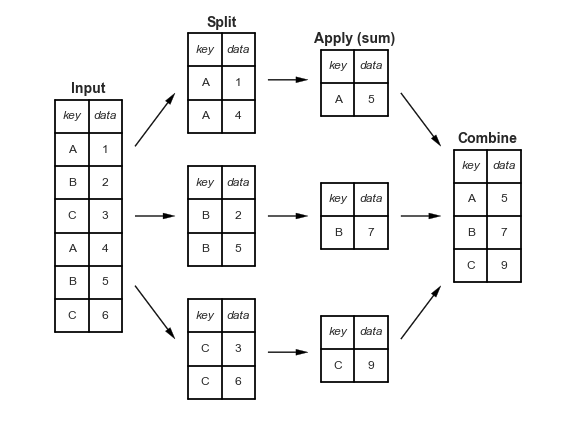
\includegraphics{split_apply_combine.png}
\href{https://github.com/jakevdp/PythonDataScienceHandbook/blob/master/notebooks/03.08-Aggregation-and-Grouping.ipynb}{source}

    \[\vspace{3in}\]

    \begin{Verbatim}[commandchars=\\\{\}]
{\color{incolor}In [{\color{incolor}19}]:} \PY{c}{\PYZpc{}\PYZpc{}latex}
         \PY{k}{\PYZbs{}newpage}
\end{Verbatim}


    \newpage


    
    \hypertarget{consider-the-following-code-and-output.}{%
\subsection{Consider the following code and
output.}\label{consider-the-following-code-and-output.}}

    \begin{Verbatim}[commandchars=\\\{\}]
{\color{incolor}In [{\color{incolor}15}]:} \PY{n}{df}\PY{p}{[}\PY{l+s+s1}{\PYZsq{}}\PY{l+s+s1}{adult}\PY{l+s+s1}{\PYZsq{}}\PY{p}{]} \PY{o}{=} \PY{n}{df}\PY{p}{[}\PY{l+s+s1}{\PYZsq{}}\PY{l+s+s1}{age}\PY{l+s+s1}{\PYZsq{}}\PY{p}{]}\PY{o}{\PYZgt{}}\PY{o}{=}\PY{l+m+mi}{18}
         \PY{n}{survivors\PYZus{}cube} \PY{o}{=} \PY{n}{df}\PY{o}{.}\PY{n}{pivot\PYZus{}table}\PY{p}{(}
             \PY{n}{index}\PY{o}{=}\PY{l+s+s2}{\PYZdq{}}\PY{l+s+s2}{sex}\PY{l+s+s2}{\PYZdq{}}\PY{p}{,} \PY{n}{columns}\PY{o}{=}\PY{p}{[}\PY{l+s+s2}{\PYZdq{}}\PY{l+s+s2}{adult}\PY{l+s+s2}{\PYZdq{}}\PY{p}{,} \PY{l+s+s2}{\PYZdq{}}\PY{l+s+s2}{pclass}\PY{l+s+s2}{\PYZdq{}}\PY{p}{]}\PY{p}{,}
             \PY{n}{values}\PY{o}{=}\PY{l+s+s2}{\PYZdq{}}\PY{l+s+s2}{survived}\PY{l+s+s2}{\PYZdq{}}\PY{p}{,} \PY{n}{aggfunc}\PY{o}{=}\PY{n}{np}\PY{o}{.}\PY{n}{mean}\PY{p}{)}
         \PY{n}{table} \PY{o}{=} \PY{p}{(}\PY{n}{survivors\PYZus{}cube}\PY{o}{*}\PY{l+m+mi}{10}\PY{p}{)}\PY{o}{.}\PY{n}{round}\PY{p}{(}\PY{p}{)}\PY{o}{.}\PY{n}{astype}\PY{p}{(}\PY{n+nb}{int}\PY{p}{)}
         \PY{n}{table}
\end{Verbatim}


\begin{Verbatim}[commandchars=\\\{\}]
{\color{outcolor}Out[{\color{outcolor}15}]:} adult  False        True       
         pclass     1   2  3     1  2  3
         sex                            
         female     9  10  5    10  9  4
         male       4   5  1     3  1  2
\end{Verbatim}
            
    From the above data, what is the result of \texttt{table.stack()}.

    \[\vspace{2in}\]

    \hypertarget{given-the-following}{%
\subsection{Given the following:}\label{given-the-following}}

    \begin{Verbatim}[commandchars=\\\{\}]
{\color{incolor}In [{\color{incolor}18}]:} \PY{n}{adult\PYZus{}pclass\PYZus{}counts} \PY{o}{=} \PY{n}{pd}\PY{o}{.}\PY{n}{crosstab}\PY{p}{(}\PY{n}{df}\PY{o}{.}\PY{n}{pclass}\PY{p}{,} \PY{n}{df}\PY{o}{.}\PY{n}{adult}\PY{p}{)}
         \PY{n}{adult\PYZus{}pclass\PYZus{}counts}
\end{Verbatim}


\begin{Verbatim}[commandchars=\\\{\}]
{\color{outcolor}Out[{\color{outcolor}18}]:} adult   False  True 
         pclass              
         1          54    269
         2          49    228
         3         314    395
\end{Verbatim}
            
    \begin{Verbatim}[commandchars=\\\{\}]
{\color{incolor}In [{\color{incolor}22}]:} \PY{n}{adult} \PY{o}{=} \PY{n}{adult\PYZus{}pclass\PYZus{}counts}\PY{o}{.}\PY{n}{sum}\PY{p}{(}\PY{n}{axis}\PY{o}{=}\PY{l+m+mi}{0}\PY{p}{)} \PY{o}{/} \PY{n}{N}
         \PY{n}{adult}
\end{Verbatim}


\begin{Verbatim}[commandchars=\\\{\}]
{\color{outcolor}Out[{\color{outcolor}22}]:} adult
         False    0.318564
         True     0.681436
         dtype: float64
\end{Verbatim}
            
    \begin{Verbatim}[commandchars=\\\{\}]
{\color{incolor}In [{\color{incolor}23}]:} \PY{n}{pclass} \PY{o}{=} \PY{n}{adult\PYZus{}pclass\PYZus{}counts}\PY{o}{.}\PY{n}{sum}\PY{p}{(}\PY{n}{axis}\PY{o}{=}\PY{l+m+mi}{1}\PY{p}{)} \PY{o}{/} \PY{n}{N}
         \PY{n}{pclass}
\end{Verbatim}


\begin{Verbatim}[commandchars=\\\{\}]
{\color{outcolor}Out[{\color{outcolor}23}]:} pclass
         1    0.246753
         2    0.211612
         3    0.541635
         dtype: float64
\end{Verbatim}
            
    \begin{Verbatim}[commandchars=\\\{\}]
{\color{incolor}In [{\color{incolor}24}]:} \PY{n}{N} \PY{o}{=} \PY{n}{adult\PYZus{}pclass\PYZus{}counts}\PY{o}{.}\PY{n}{sum}\PY{p}{(}\PY{p}{)}\PY{o}{.}\PY{n}{sum}\PY{p}{(}\PY{p}{)}
         \PY{n}{joint} \PY{o}{=} \PY{n}{adult\PYZus{}pclass\PYZus{}counts} \PY{o}{/} \PY{n}{N}
         \PY{n}{display}\PY{p}{(}\PY{n}{joint}\PY{p}{)}
         \PY{n}{expected} \PY{o}{=} \PY{n}{np}\PY{o}{.}\PY{n}{outer}\PY{p}{(}\PY{n}{pclass}\PY{p}{,} \PY{n}{adult}\PY{p}{)}
         \PY{n}{display}\PY{p}{(}\PY{n}{expected}\PY{p}{)}
\end{Verbatim}


    
    \begin{verbatim}
adult      False     True 
pclass                    
1       0.041253  0.205500
2       0.037433  0.174179
3       0.239878  0.301757
    \end{verbatim}

    
    
    \begin{verbatim}
array([[ 0.07860665,  0.1681466 ],
       [ 0.06741189,  0.14420002],
       [ 0.17254525,  0.36908959]])
    \end{verbatim}

    
    \[\noindent\]\textbf{What is the code for calculating Chi-square?}

\[\noindent\]\textbf{Chi-square distance} solves the problem of total
variation distance by dividing by the difference by expected proportion,
effectively calculating the \emph{relative} difference between the two
proportions:

\[ \chi^2 = \sum_{\text{A, B}} \frac{(P(A \text{ and } B) - P(A) P(B))^2}{P(A) P(B)}. \]

    \[\vspace{3in}\]

    \hypertarget{what-is-the-difference-between-covariance-and-correlation-why-would-you-want-to-look-at-one-or-the-other}{%
\subsubsection{What is the difference between covariance and
correlation? Why would you want to look at one or the
other?}\label{what-is-the-difference-between-covariance-and-correlation-why-would-you-want-to-look-at-one-or-the-other}}

    \[\vspace{2in}\]

    \hypertarget{points-the-table-below-is-a-sample-from-a-dataset-used-to-help-determine-if-a-house-is-acceptable-to-purchase.-calculate-pacceptableyesnot-included3new-using-the-naive-bayes-classifier-described-in-class.}{%
\subsection{\texorpdfstring{(10 points) The table below is a sample from
a dataset used to help determine if a house is acceptable to purchase.
Calculate \texttt{P(Acceptable=Yes\textbar{}Not\ included,3,New)} using
the naive Bayes classifier described in
class.}{(10 points) The table below is a sample from a dataset used to help determine if a house is acceptable to purchase. Calculate P(Acceptable=Yes\textbar{}Not included,3,New) using the naive Bayes classifier described in class.}}\label{points-the-table-below-is-a-sample-from-a-dataset-used-to-help-determine-if-a-house-is-acceptable-to-purchase.-calculate-pacceptableyesnot-included3new-using-the-naive-bayes-classifier-described-in-class.}}

    \begin{table}[!h]
    \centering
    \begin{tabular}{lllll}
    House & Furniture  & \# Rooms & Kitchen & Acceptable \\
    1     & Not included & 3         & New       & Yes          \\
    2     & Included     & 3         & Old       & No           \\
    3     & Not included & 4         & Old       & Yes          \\
    4     & Not included & 3         & New       & No           \\
    5     & Included     & 4         & Old       & Yes          \\
    \end{tabular}
\end{table}

    \[\vspace{4in}\]

    \hypertarget{points-find-the-eigenvalues-and-eigenvectors-of-the-following-covariance-matrix-circle-answer.-show-your-work.}{%
\subsection{(10 points) Find the eigenvalues and eigenvectors of the
following covariance matrix (circle answer). Show your
work.}\label{points-find-the-eigenvalues-and-eigenvectors-of-the-following-covariance-matrix-circle-answer.-show-your-work.}}

    \begin{Verbatim}[commandchars=\\\{\}]
{\color{incolor}In [{\color{incolor}17}]:} \PY{c}{\PYZpc{}\PYZpc{}latex}
          \PY{l+s+sb}{\PYZbs{}[}
         \PY{n+nb}{   }\PY{n+nv}{\PYZbs{}Sigma}\PY{o}{=}
         \PY{n+nb}{  }\PY{n+nv}{\PYZbs{}left}\PY{o}{[}\PY{n+nb}{ }\PY{n+nb}{\PYZob{}}\PY{n+nv}{\PYZbs{}begin}\PY{n+nb}{\PYZob{}}\PY{n+nb}{array}\PY{n+nb}{\PYZcb{}}\PY{n+nb}{\PYZob{}}\PY{n+nb}{cc}\PY{n+nb}{\PYZcb{}}
         \PY{n+nb}{   }\PY{l+m}{4}\PY{n+nb}{ }\PY{n+nb}{\PYZam{}}\PY{n+nb}{ }\PY{l+m}{2}\PY{n+nb}{ }\PY{n+nv}{\PYZbs{}\PYZbs{}}
         \PY{n+nb}{   }\PY{l+m}{2}\PY{n+nb}{ }\PY{n+nb}{\PYZam{}}\PY{n+nb}{ }\PY{l+m}{4}\PY{n+nb}{ }\PY{n+nv}{\PYZbs{}\PYZbs{}}
         \PY{n+nb}{  }\PY{n+nv}{\PYZbs{}end}\PY{n+nb}{\PYZob{}}\PY{n+nb}{array}\PY{n+nb}{\PYZcb{}}\PY{n+nb}{ }\PY{n+nb}{\PYZcb{}}\PY{n+nb}{ }\PY{n+nv}{\PYZbs{}right}\PY{o}{]}
         \PY{l+s}{\PYZbs{}]}
\end{Verbatim}


     \[
   \Sigma=
  \left[ {\begin{array}{cc}
   4 & 2 \\
   2 & 4 \\
  \end{array} } \right]
\]


    
    \[\vspace{3in}\]

    \hypertarget{points-what-is-the-percent-variance-explained-in-pc2-using-your-results-from-the-last-question}{%
\subsection{(5 points) What is the percent variance explained in PC2
using your results from the last
question?}\label{points-what-is-the-percent-variance-explained-in-pc2-using-your-results-from-the-last-question}}

    \[\vspace{2in}\]


    % Add a bibliography block to the postdoc
    
    
    
    \end{document}
